% !BIB program = bibtex
\documentclass[aspectratio=169,10pt]{beamer}

% Required packages
\usepackage[english]{babel}
\usepackage[utf8]{inputenc}
\usepackage{graphicx}
% Plots are generated into ../output/plots by the R pipeline.
% Paths below are written relative to that folder (e.g. plots/age_histogram.pdf).
\graphicspath{{../output/}{./}}
\usepackage{booktabs}
\usepackage{xcolor}
\usepackage{amsmath}
\usepackage{hyperref}
\usepackage{tikz}
\usetikzlibrary{positioning,shapes,arrows,fit,calc,backgrounds}
\usepackage{pgfplots}
\pgfplotsset{compat=1.18}
\usepackage{csquotes}
\usepackage{caption}

% Bibliography (Biber backend)
\usepackage[backend=biber,style=authoryear,natbib=true]{biblatex}
\addbibresource{references.bib}

% Define modern color scheme (from template)
\definecolor{fuBlue}{RGB}{0, 51, 102}
\definecolor{accentColor}{RGB}{204, 153, 0}
\definecolor{bgColor}{RGB}{248, 248, 248}
\definecolor{textColor}{RGB}{51, 51, 51}

% Custom Metropolis theme setup
\usetheme{metropolis}
\setbeamercolor{background canvas}{bg=bgColor}
\setbeamercolor{normal text}{fg=textColor}
\setbeamercolor{frametitle}{bg=fuBlue, fg=white}
\setbeamercolor{title}{bg=white, fg=fuBlue}
\setbeamercolor{section in toc}{fg=fuBlue}
\setbeamercolor{subsection in toc}{fg=fuBlue}
\setbeamercolor{block title}{bg=fuBlue, fg=white}
\setbeamercolor{block body}{bg=bgColor, fg=textColor}
\setbeamercolor{alerted text}{fg=accentColor}
\setbeamercolor{itemize item}{fg=fuBlue}
\setbeamercolor{itemize subitem}{fg=accentColor}
\setbeamercolor{enumerate item}{fg=fuBlue}
\setbeamercolor{button}{bg=accentColor, fg=white}

\setbeamerfont{title}{size=\Large, series=\bfseries}
\setbeamerfont{subtitle}{size=\large}
\setbeamerfont{frametitle}{size=\large, series=\bfseries}
\setbeamerfont{block title}{size=\normalsize, series=\bfseries}

\setbeamertemplate{navigation symbols}{}
\setbeamertemplate{caption}[numbered]
\setbeamertemplate{itemize items}[circle]
\setbeamertemplate{itemize subitem}[triangle]
\setbeamertemplate{enumerate items}[default]
\setbeamertemplate{footline}[frame number]
\setbeamertemplate{section in toc}[sections numbered]

% Title page information
\title{German Lexicon Project -- Final Dataset}
\author{Aliona Petrenco, Louis Schiekiera, \& Fritz Günther}
\institute{Humboldt-Universit\"at zu Berlin}
\date{June 03, 2026}

\begin{document}

% ===================================================================
% TITLE SLIDE
% ===================================================================
\begin{frame}[plain]
    \begin{tikzpicture}[remember picture, overlay]
        \fill[fuBlue] (current page.north west) rectangle ([yshift=-1cm]current page.north east);
        \fill[white] ([yshift=-1cm]current page.north west) rectangle (current page.south east);
    \end{tikzpicture}

    \vspace{0.5cm}

    \begin{center}
        {\usebeamercolor[fg]{title}\usebeamerfont{title}\large\textbf{\inserttitle}}\par
        \vspace{1em}

        \begin{minipage}{0.85\textwidth}
            \centering
            {\usebeamerfont{author}\insertauthor}\par
            \vspace{0.2em}
            {\color{fuBlue}\rule{0.3\textwidth}{0.5pt}}\par
            \vspace{0.2em}
            {\usebeamerfont{institute}\footnotesize\insertinstitute}
        \end{minipage}

        \vspace{0.5cm}

        
\begin{tikzpicture}
            \node[draw=fuBlue, thick, fill=bgColor, rounded corners, text width=0.5\textwidth, align=center, inner sep=6pt] {
                \color{fuBlue}\textbf{TRUST Analysis Meeting}\\
                \small\textcolor{textColor}{Online, June 03, 2026}
            };
        \end{tikzpicture}
    \end{center}
\end{frame}


\begin{frame}
    \frametitle{Recap: Design Overview}
    \begin{columns}
        \begin{column}{0.55\textwidth}
            \begin{block}{Stimuli}
                \begin{itemize}
                    \item \textbf{60,000} total items
                    \begin{itemize}
                        \item 30,000 words
                        \item 30,000 nonwords
                    \end{itemize}
                    \item \textbf{30 repetitions} per item
                    \item Resulting in \textbf{1.8\,M trials} total
                \end{itemize}
            \end{block}
            \begin{block}{Participants}
                \begin{itemize}
                    \item Target: \textbf{1,440} participants
                    \item \textbf{1,250 trials} per participant
                    \item 10 blocks of 125 trials
                \end{itemize}
            \end{block}
        \end{column}
        \begin{column}{0.42\textwidth}

            \begin{alertblock}{Exclusion Criteria}
                \begin{enumerate}
                    \item Aborted experiments
                    \item Incomplete data due to technical issues (missing blocks or trials)
                    \item Non-native German speakers
                    \item Lexical decision accuracy $< 75$\%
                    \item Underage participants ($< 18$ years)
                \end{enumerate}
            \end{alertblock}
        \end{column}
    \end{columns}

\end{frame}


% ===================================================================
% SECTION: PROGRESS VISUALIZATION
% ===================================================================


\begin{frame}
    \frametitle{Overall Progress: Data Collection Complete}
    \begin{center}
        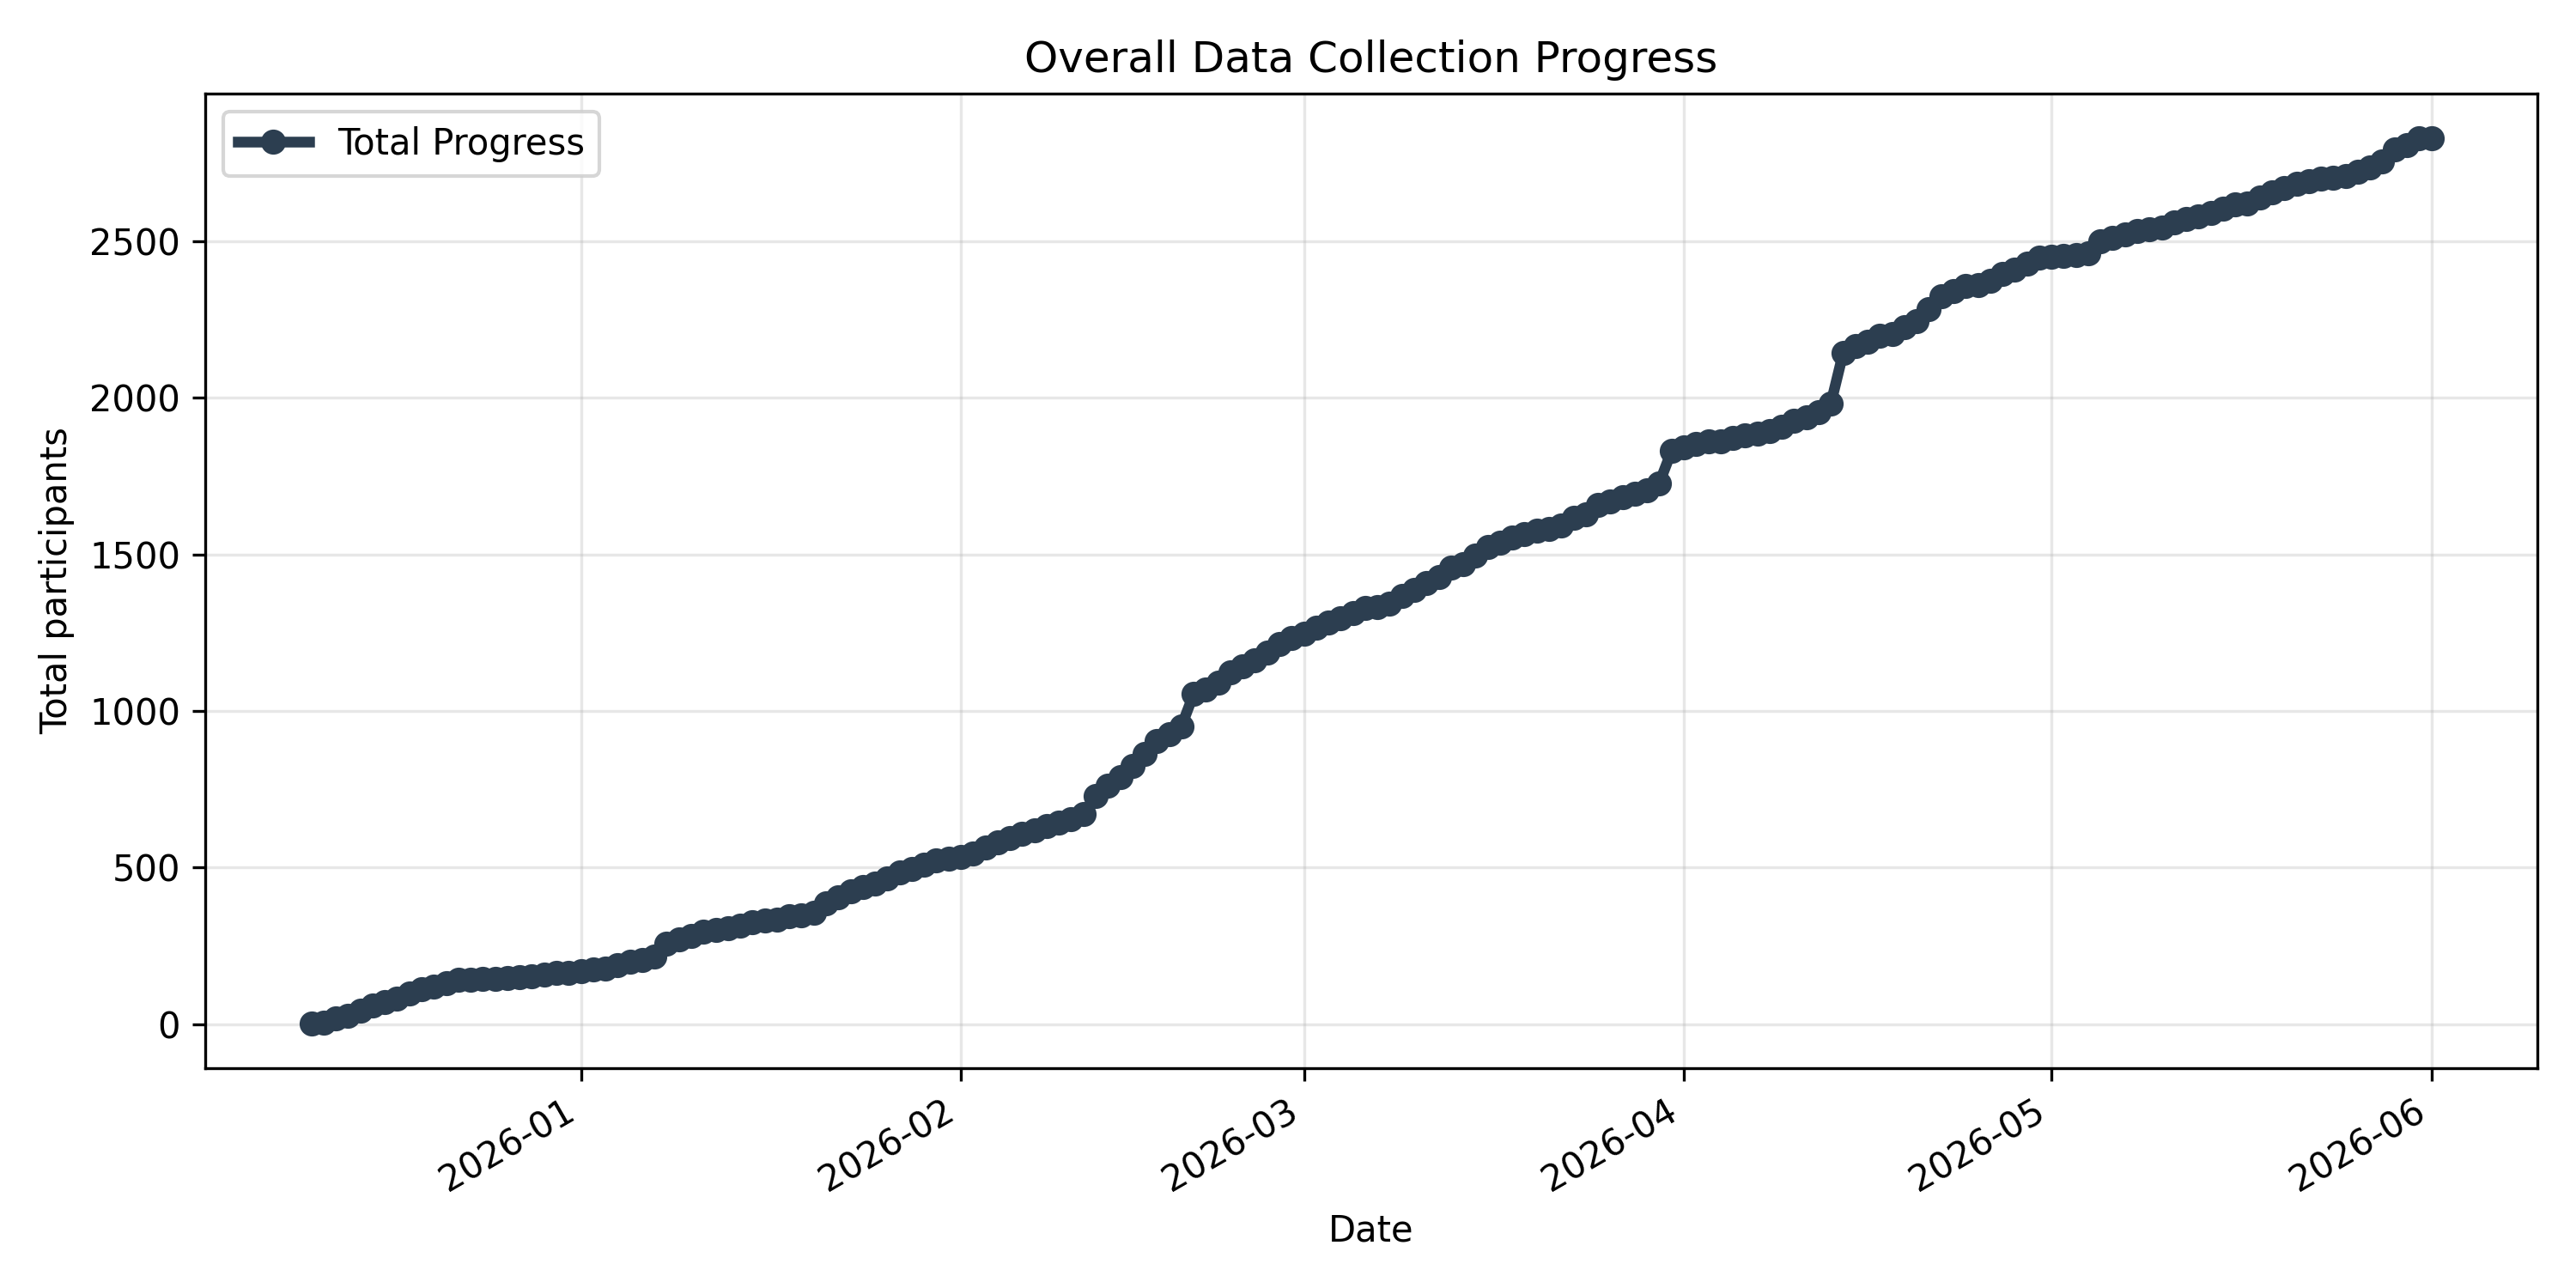
\includegraphics[width=0.75\textwidth]{plots/data_collection/overall_progress.png}
        \captionof{figure}{Cumulative data collection from December 2025 onward. Data collection is now \textbf{complete}: as of June 1, 2026, \emph{n} = \textbf{2,825} datasets were collected.
        }

\end{center}

\end{frame}

\begin{frame}
    \frametitle{New Datasets per Day}
    \begin{center}
        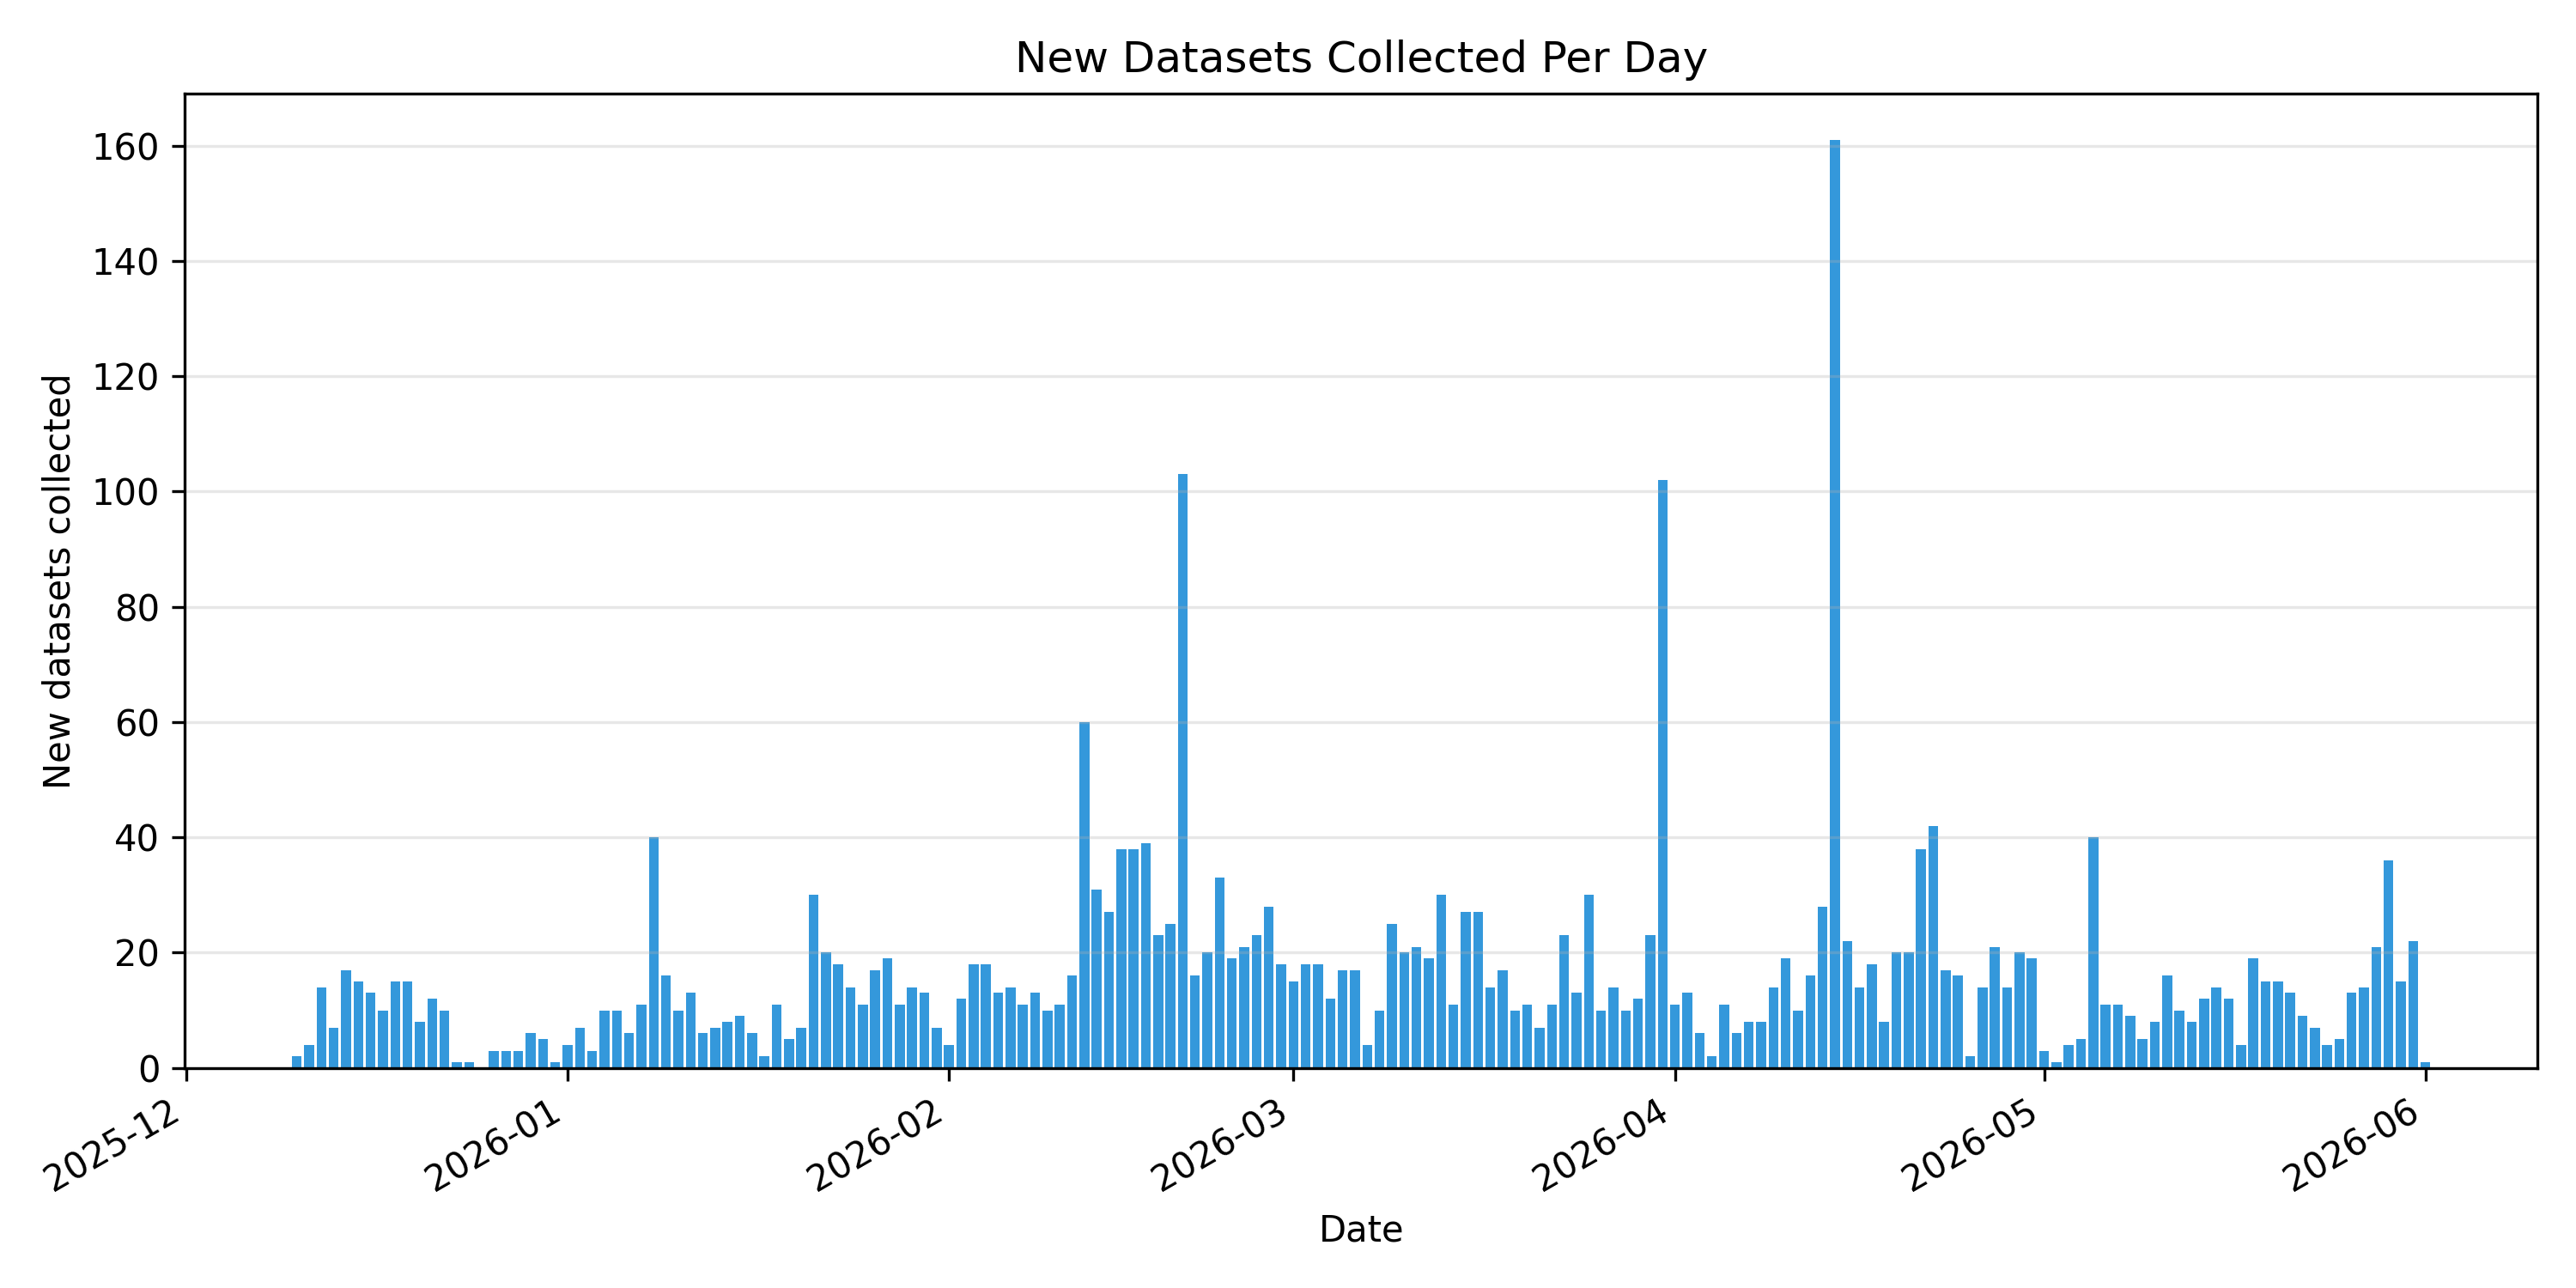
\includegraphics[width=0.75\textwidth]{plots/data_collection/new_datasets_per_day.png}
        \captionof{figure}{New datasets collected per day, from December 2025 to completion in June 2026.}
    \end{center}
\end{frame}





% ===================================================================
% SECTION: DATA CLEANING & CURRENT STATUS
% ===================================================================

\begin{frame}
    \frametitle{Data Cleaning Pipeline}
    \begin{center}
        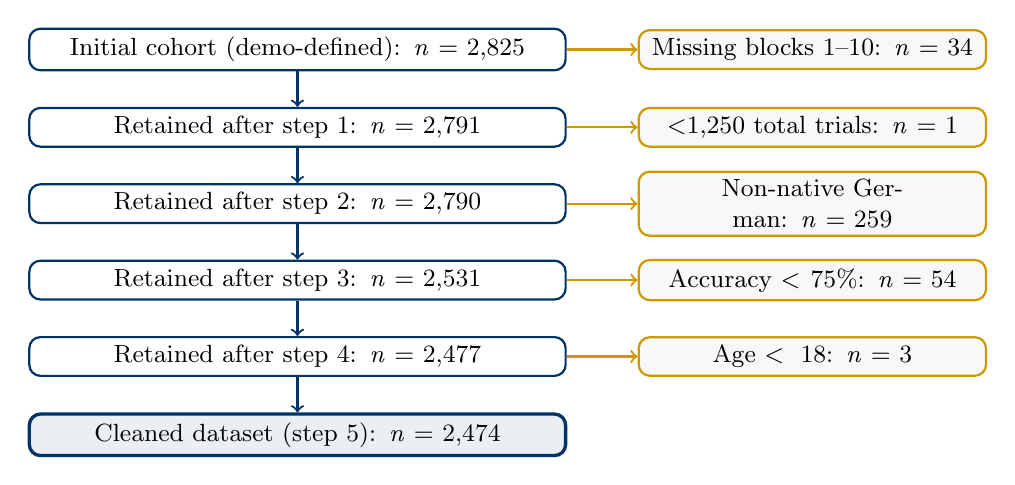
\begin{tikzpicture}[
            node distance=0.45cm and 0.9cm,
            main/.style={draw=fuBlue, rounded corners, thick, fill=white, align=center, text width=6.6cm, inner sep=3pt, font=\small},
            excl/.style={draw=accentColor, rounded corners, thick, fill=bgColor, align=center, text width=4.2cm, inner sep=3pt, font=\small},
            final/.style={draw=fuBlue, rounded corners, very thick, fill=fuBlue!8, align=center, text width=6.6cm, inner sep=3pt, font=\small}
        ]
            \node[main] (s1) {Initial cohort (demo-defined): \emph{n} = 2,825};
            \node[main, below=of s1] (s2) {Retained after step 1: \emph{n} = 2,791};
            \node[main, below=of s2] (s3) {Retained after step 2: \emph{n} = 2,790};
            \node[main, below=of s3] (s4) {Retained after step 3: \emph{n} = 2,531};
            \node[main, below=of s4] (s5) {Retained after step 4: \emph{n} = 2,477};
            \node[final, below=of s5] (s6) {Cleaned dataset (step 5): \emph{n} = 2,474};

            \node[excl, right=of s1] (e1) {Missing blocks 1--10: \emph{n} = 34};
            \node[excl, right=of s2] (e2) {$<$1,250 total trials: \emph{n} = 1};
            \node[excl, right=of s3] (e3) {Non-native German: \emph{n} = 259};
            \node[excl, right=of s4] (e4) {Accuracy $< 75\%$: \emph{n} = 54};
            \node[excl, right=of s5] (e5) {Age $< 18$: \emph{n} = 3};

            \draw[->, thick, fuBlue] (s1) -- (s2);
            \draw[->, thick, fuBlue] (s2) -- (s3);
            \draw[->, thick, fuBlue] (s3) -- (s4);
            \draw[->, thick, fuBlue] (s4) -- (s5);
            \draw[->, thick, fuBlue] (s5) -- (s6);

            \draw[->, thick, accentColor] (s1.east) -- (e1.west);
            \draw[->, thick, accentColor] (s2.east) -- (e2.west);
            \draw[->, thick, accentColor] (s3.east) -- (e3.west);
            \draw[->, thick, accentColor] (s4.east) -- (e4.west);
            \draw[->, thick, accentColor] (s5.east) -- (e5.west);
        \end{tikzpicture}
    \end{center}
\end{frame}



\begin{frame}
    \frametitle{Final Sample Overview}
    \begin{columns}
        \begin{column}{0.4\textwidth}
            \begin{block}{Final Counts (Jun 1, 2026)}
                \begin{itemize}
                    \item Datasets collected: \textbf{2,825}
                    \item Retained after cleaning: \textbf{2,474}
                    \item Exclusion rate: \textbf{12.4\%}
                    \item Cleaned trials: \textbf{3,097,500}
                \end{itemize}
            \end{block}
        \end{column}
        \begin{column}{0.6\textwidth}
            \begin{block}{Target \& Coverage}
                \begin{tabular}{lr}
                    \toprule
                    Metric & Value \\
                    \midrule
                    Original target (valid) & 1,440 \\
                    Final retained          & 2,474 \\
                    Stimulus-list coverage  & complete \\
                    \bottomrule
                \end{tabular}
            \end{block}
            \vspace{0.3cm}
            \begin{alertblock}{Status}
                \begin{itemize}
                    \item Data collection \textbf{complete} (Jun 1, 2026); recruitment closed
                \end{itemize}
            \end{alertblock}

        
        \end{column}
    \end{columns}
\end{frame}


% ===================================================================
% SECTION: PRELIMINARY DATA ANALYSIS
% ===================================================================

\begin{frame}
    \frametitle{Demographics \& Participant Overview}
    \begin{columns}
        \begin{column}{0.48\textwidth}
            \vspace{-0.5cm}

            \begin{block}{Gender}
                \begin{tabular}{lrr}
                    \toprule
                    & $n$ & \% \\
                    \midrule
                    Female    & 1,776 & 71.8 \\
                    Male      & 662   & 26.8 \\
                    Diverse   & 27    & 1.1 \\
                    No answer & 9     & 0.4 \\
                    \bottomrule
                \end{tabular}
            \end{block}
            \begin{block}{Education}
                \begin{tabular}{lrr}
                    \toprule
                    & $n$ & \% \\
                    \midrule
                    Abitur/Fachabitur & 1,603 & 64.8 \\
                    University degree & 617   & 24.9 \\
                    Vocational        & 221   & 8.9 \\
                    Other             & 33    & 1.3 \\
                    \bottomrule
                \end{tabular}
            \end{block}

        \end{column}
        \begin{column}{0.48\textwidth}
    
            \begin{block}{Age}
                \begin{center}
                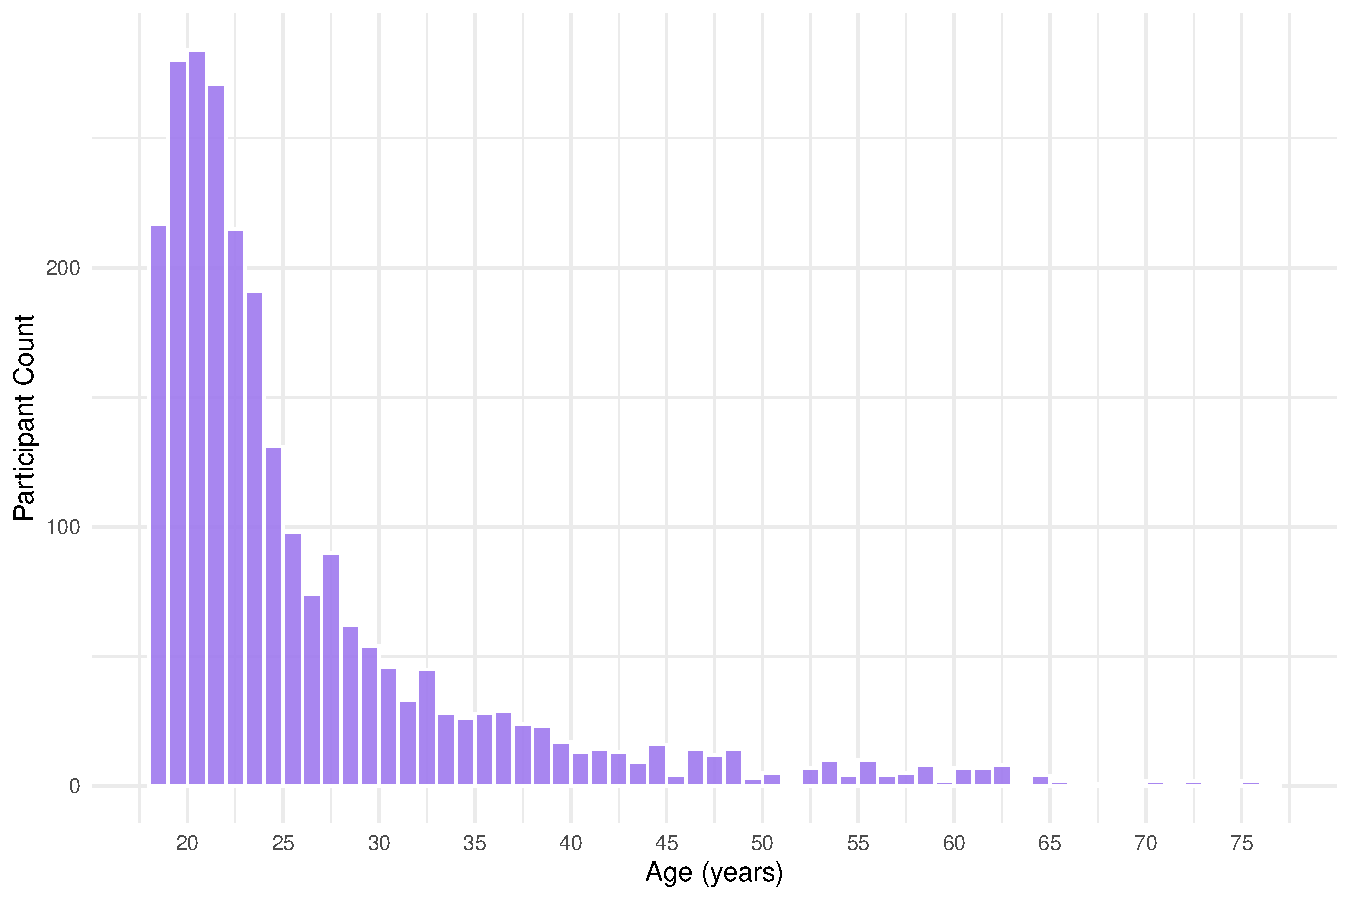
\includegraphics[width=0.75\textwidth]{plots/age_histogram.pdf}
                \captionof{figure}{Distribution of age from \emph{n} = 2,472 participants. $M (SD) = 26.7 (9.37)$, $Mdn = 23$.}
                \end{center}
            \end{block}
            \vspace{-0.5cm}
            \begin{block}{Language Background}
                \begin{itemize}
                    \item Early multilingual: 336 (13.6\%)
                    \item Currently multilingual: 2,251 (91.0\%)
                \end{itemize}
            \end{block}

        \end{column}
    \end{columns}
\end{frame}



\begin{frame}
    \frametitle{Geographic Distribution}
    \begin{columns}
        \begin{column}{0.4\textwidth}
            \vspace{-0.5cm}

            \begin{block}{Where did participants grow up?}
                \begin{tabular}{lrrr}
                    \toprule
                    Country & $n$  &\% \\
                    \midrule
                      Germany      &      2,262    & 91.4 \\
                      Austria            & 99    & 4.0 \\
                      Switzerland        & 76    & 3.1 \\
                      Other              & 37    & 1.5 \\
                    \bottomrule
                \end{tabular}
            \end{block}

        \end{column}
        \begin{column}{0.6\textwidth}
    
                \begin{center}
                \includegraphics[width=\textwidth]{plots/german_origin_plz_map.pdf}
                \captionof{figure}{Distribution of postal codes from \emph{n} = 2,262 participants in Germany.}
                \end{center}


        \end{column}
    \end{columns}
\end{frame}

\begin{frame}
    \frametitle{Accuracy by Participant}
    \begin{columns}
        \begin{column}{0.3\textwidth}
            \begin{block}{Descriptive Statistics}
                \begin{tabular}{lr}
                    \toprule
                    Statistic & Value (\%) \\
                    \midrule
                    $M$        & 92.9 \\
                    $\mathit{SD}$  & 6.7 \\
                    $\mathit{Mdn}$ & 94.4 \\
                    Min        & 3.8 \\
                    Max        & 99.4 \\
                    \bottomrule
                \end{tabular}
            \end{block}
            \vspace{0.3cm}
            \begin{block}{By Stimulus Type}
                \begin{tabular}{lr}
                    \toprule
                    Type & Accuracy (\%) \\
                    \midrule
                    Words      & 92.4 \\
                    Pseudowords & 93.3 \\
                    \bottomrule
                \end{tabular}
            \end{block}
        \end{column}
        \begin{column}{0.60\textwidth}
            \begin{center}
                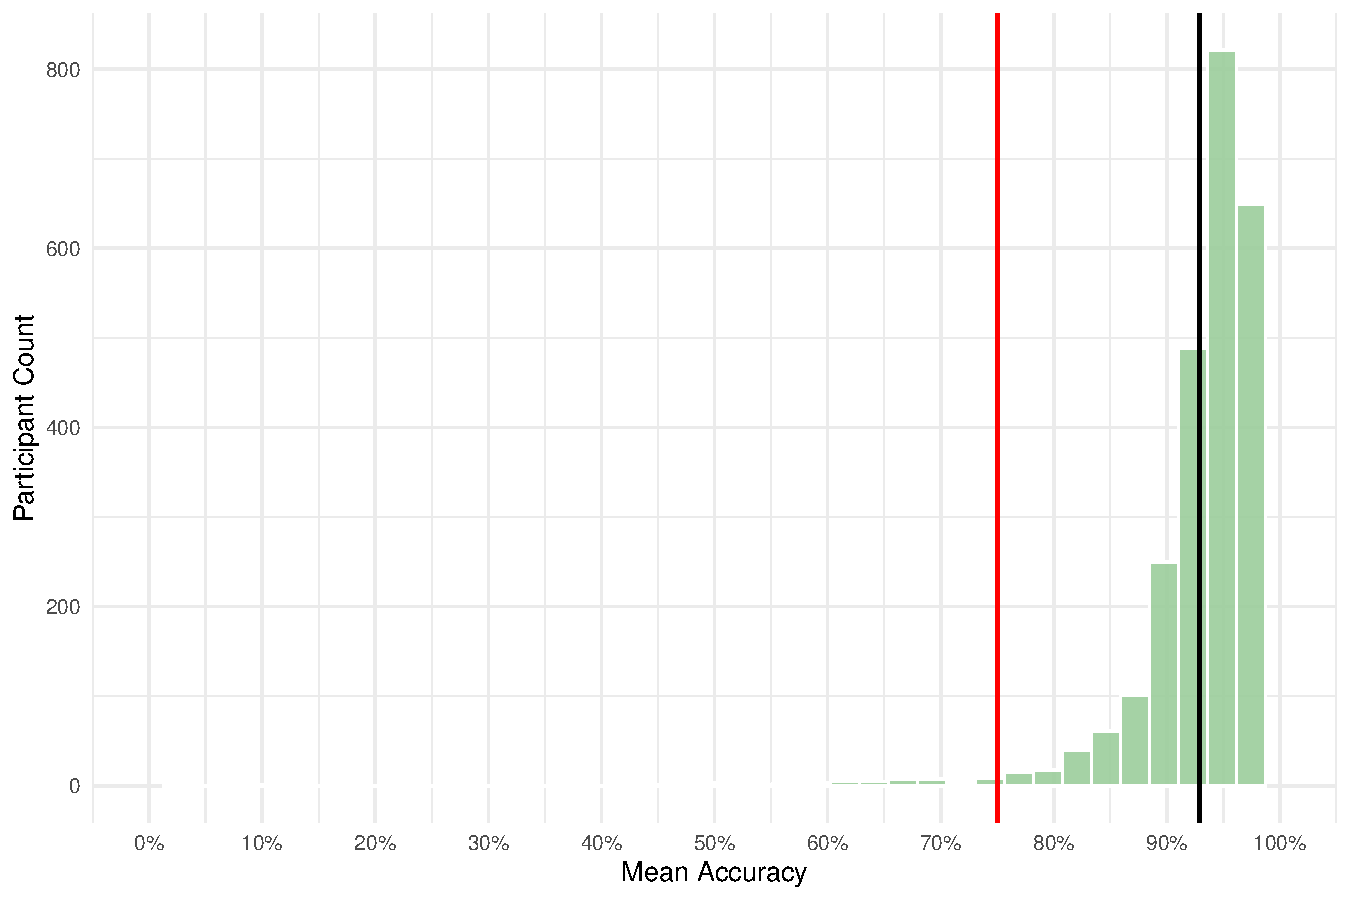
\includegraphics[width=\textwidth]{plots/accuracy_histogram.pdf}
                \captionof{figure}{Distribution of mean accuracy from \emph{n} = 2,531 participants before accuracy exclusion. Black solid line = mean, red solid line = exclusion threshold (75\%).}
            \end{center}
        \end{column}
    \end{columns}
\end{frame}

\begin{frame}
    \frametitle{Reaction Times}
    \begin{columns}
        \begin{column}{0.4\textwidth}
            \begin{block}{Overall (trimmed 200--3000\,ms)}
                \begin{tabular}{lr}
                    \toprule
                    Statistic & Value (ms) \\
                    \midrule
                    $M$            & 875 \\
                    $\mathit{Mdn}$ & 753 \\
                    $\mathit{SD}$   & 392 \\
                    \bottomrule
                \end{tabular}
            \end{block}
            \vspace{0.3cm}
            \begin{block}{By Stimulus Type}
                \begin{tabular}{lrr}
                    \toprule
                    Type & $M$ (ms) & $\mathit{Mdn}$ (ms) \\
                    \midrule
                    Words       & 817 & 715 \\
                    Pseudowords & 934 & 797 \\
                    \bottomrule
                \end{tabular}
            \end{block}
        \end{column}
        \begin{column}{0.6\textwidth}
            \begin{center}
                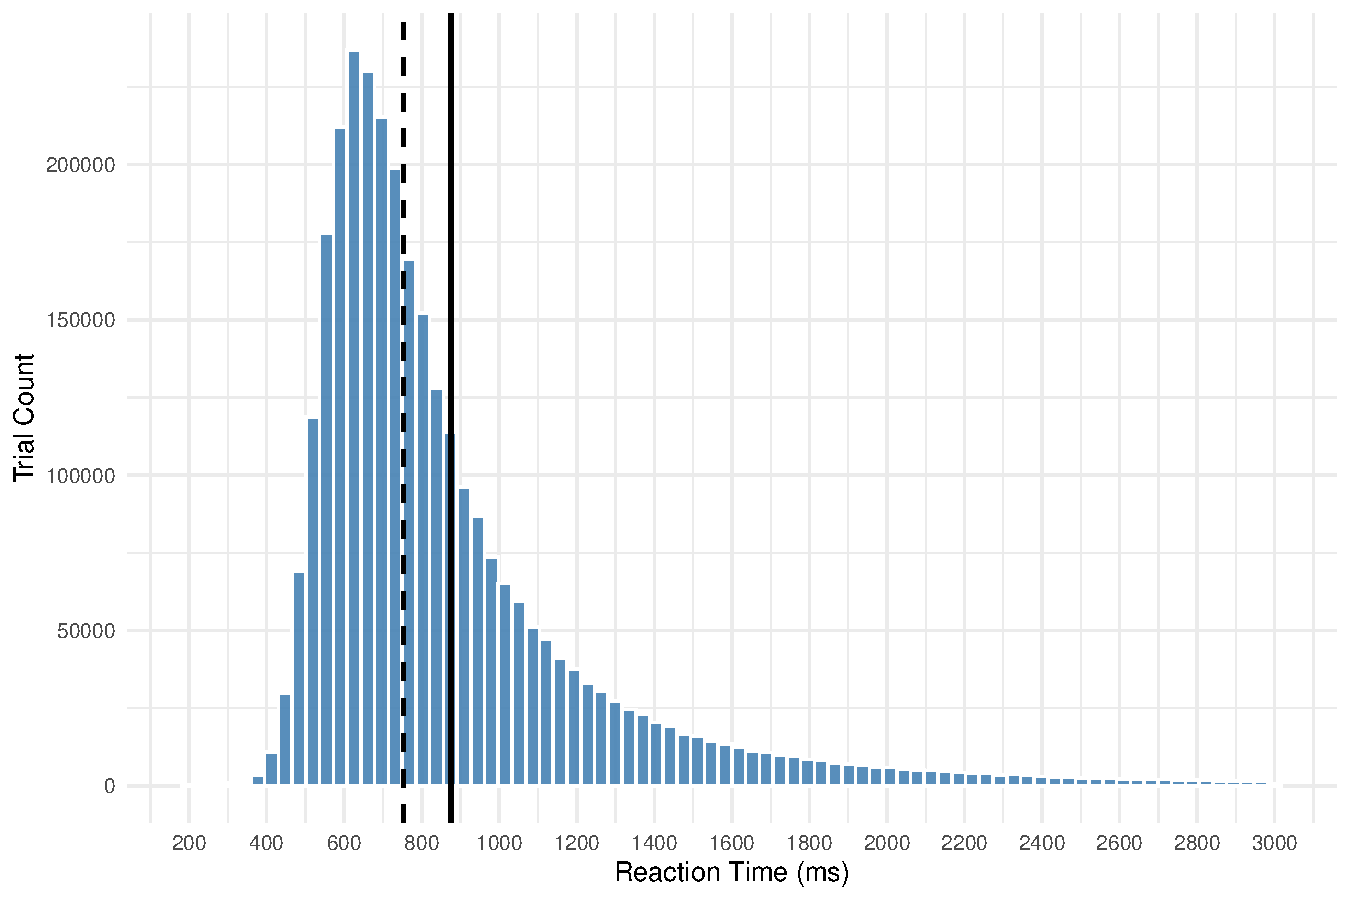
\includegraphics[width=\textwidth]{plots/rt_histogram.pdf}
                \captionof{figure}{Distribution of trimmed reaction times from \emph{n} = 2,474 participants. Solid line = mean, dashed line = median.}
            \end{center}
        \end{column}
    \end{columns}
\end{frame}

\begin{frame}
    \frametitle{RTs and Accuracy Across Blocks}
    \begin{figure}
        \centering
        \begin{minipage}{0.48\textwidth}
            \centering
            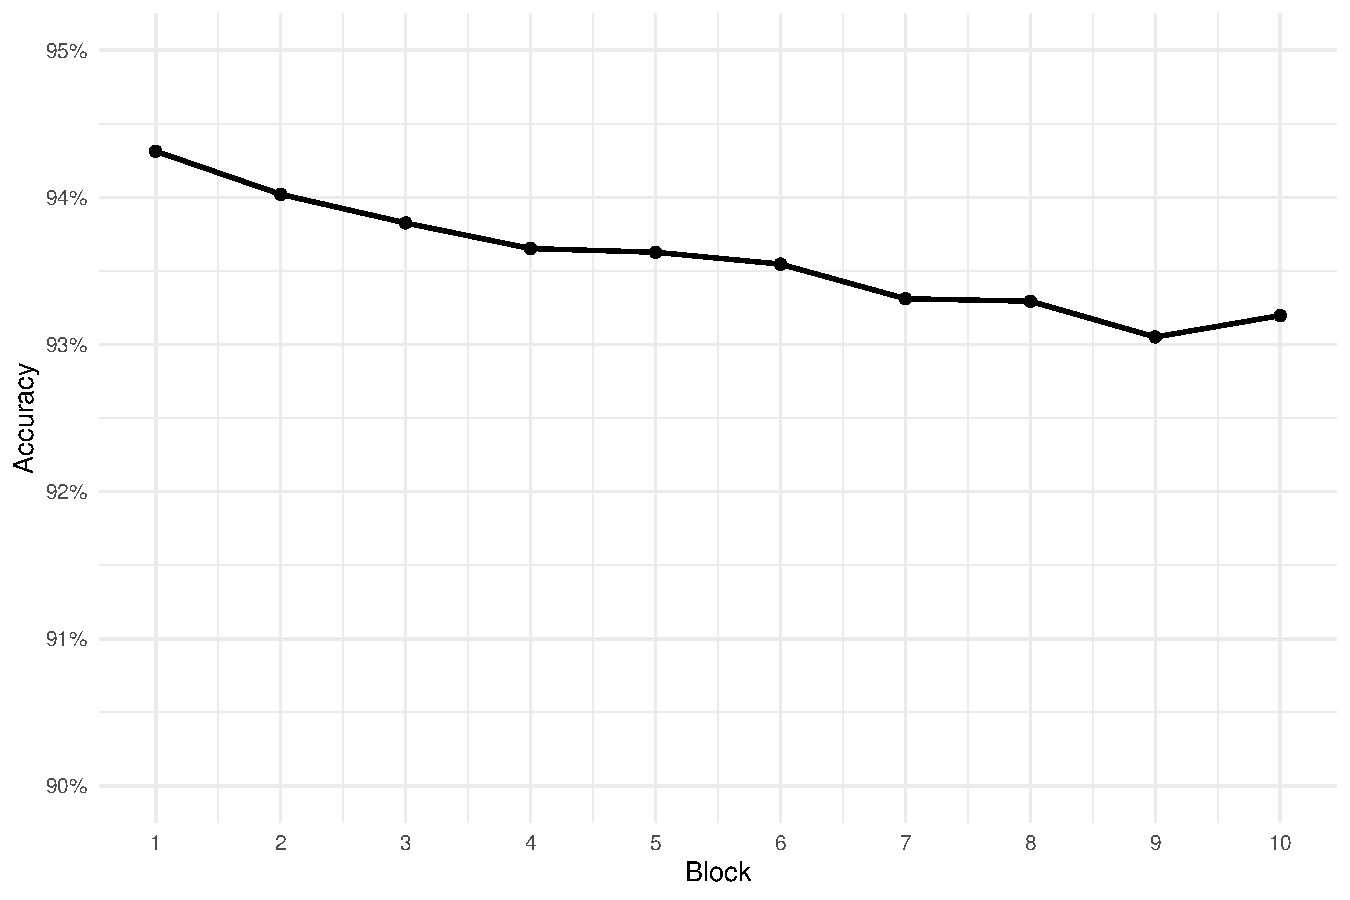
\includegraphics[width=\textwidth]{plots/accuracy_by_block.pdf}
            {\scriptsize (A)}
        \end{minipage}
        \hfill
        \begin{minipage}{0.48\textwidth}
            \centering
            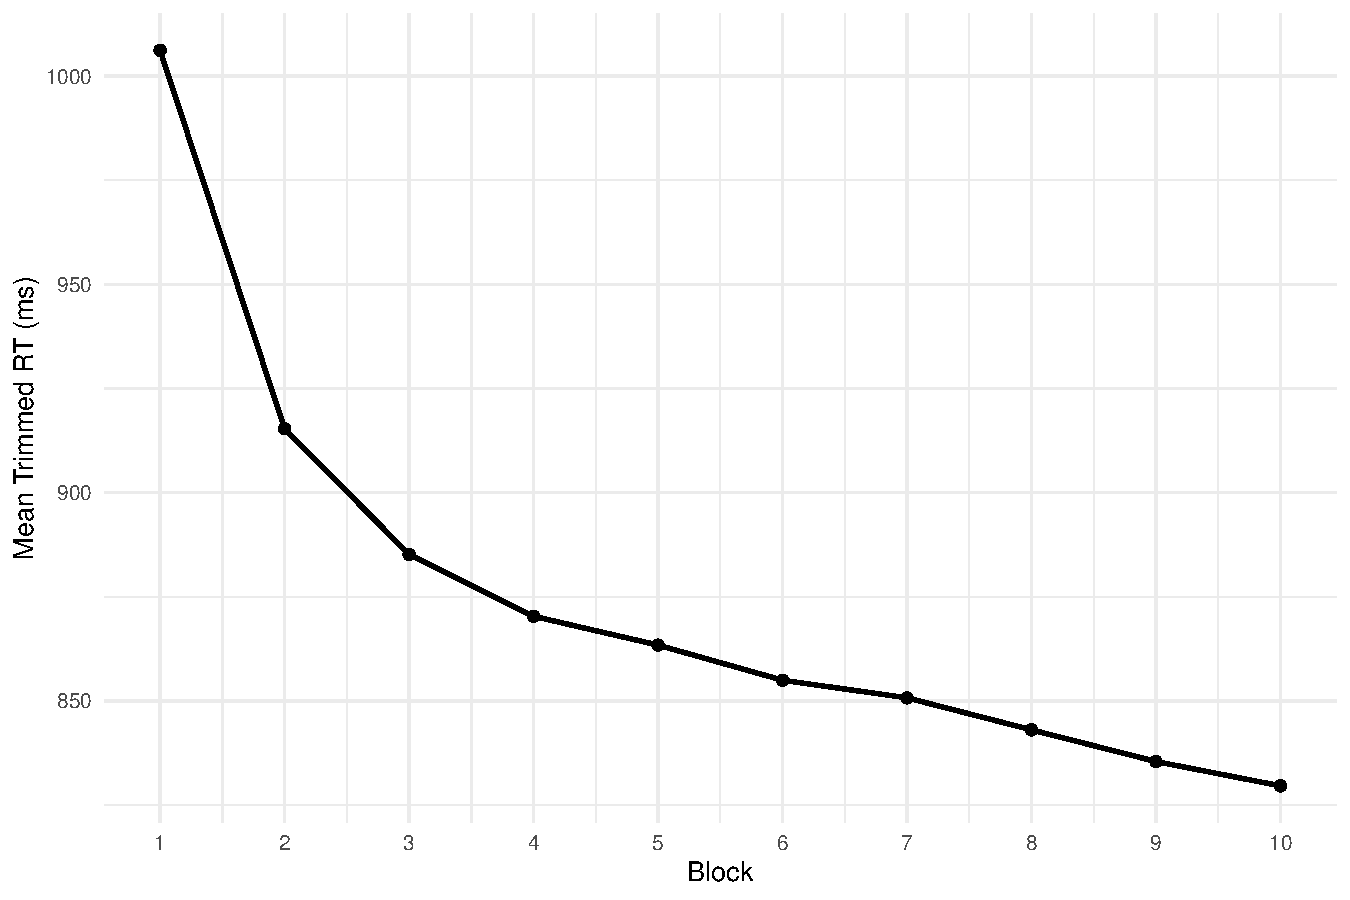
\includegraphics[width=\textwidth]{plots/rt_by_block.pdf}
            {\scriptsize (B)}
        \end{minipage}

        \caption{Performance across blocks from \emph{n} = 2,474 participants. (A) Mean accuracy per block across participants. (B) Mean reaction time per block across participants.}
    \end{figure}
\end{frame}



% ===================================================================
% SECTION: SUMMARY
% ===================================================================
\begin{frame}
    \frametitle{Summary \& Outlook}
    \begin{block}{Final Dataset}
        \begin{itemize}
            \item \textbf{2,474} participants retained after cleaning (target: 1,440 -- exceeded)
            \item \textbf{3,097,500} cleaned trials; 12.4\% participant exclusion rate
            \item Reproducible preprocessing pipeline (five exclusion steps)
        \end{itemize}
    \end{block}
    \vspace{0.3cm}
    \begin{block}{Outlook}
        \begin{itemize}
            \item Data collection \textbf{complete}; recruitment closed
            \item Reliability analyses in progress (Spearman--Brown)
            \item Prepare dataset documentation and public release
            \item Monitoring dashboard: \url{https://github.com/schiekiera/German_Lexicon_Multilab_Monitoring}
        \end{itemize}
    \end{block}
\end{frame}


\section{Thank you for your attention!}


\end{document}